%
% Slides for given talks:
%
% * 2007-02-26: PyCon 2007, Dallas (Texas), USA
%
%\documentclass[compress,trans]{beamer}
\documentclass{beamer}

\usepackage{graphicx}

\mode<presentation>
{
\usetheme{Singapore} % Singapore, default
  \setbeamertemplate{frametitle}[default][left]
  \setbeamercovered{transparent}
}

\usepackage[english]{babel}
\usepackage[latin1]{inputenc}

\usepackage{times}
\usepackage[T1]{fontenc}

\title{An extension to DBAPI 2.0 \\
for easier SQL queries}
\subtitle{}

\author{Martin Blais}

\institute{EWT LLC / Madison Tyler}

\date{http://furius.ca/antiorm/}

\subject{dbapiext presentation @ PyCon 2007}

\setcounter{tocdepth}{4}

\newcommand{\todo}[1]{}

\newcommand{\bigerror}{\begin{center}{\textbf{ERROR!}}\end{center}}

\AtBeginSubsection[]
{
  \begin{frame}<beamer>
    \frametitle{Outline}
    \tableofcontents[currentsection,currentsubsection]
  \end{frame}
}


\begin{document}

%-------------------------------------------------------------------------------
\begin{frame}
  \titlepage
\end{frame}

%===============================================================================


%-------------------------------------------------------------------------------
\begin{frame}[fragile]
  \frametitle{Introduction}

\begin{verbatim}
connection = dbapi.connect(...)
cursor = connection.cursor()

cursor.execute("""

  SELECT * FROM Users WHERE username = 'raymond'

  """)
\end{verbatim}

\end{frame}


%-------------------------------------------------------------------------------
\begin{frame}[fragile]
  \frametitle{Escaping Values}

\begin{verbatim}
name = 'raymond'
cursor.execute("""

  SELECT * FROM Users WHERE username = %s

  """, (name,))
\end{verbatim}

\vfill\pause

A common mistake is to forget to call with a tuple or a dict:
\begin{verbatim}
cursor.execute("""

  SELECT * FROM Users WHERE username = %s

  """, name)  <--- this fails
\end{verbatim}

\end{frame}


%-------------------------------------------------------------------------------
\begin{frame}[fragile]
  \frametitle{String Interpolation Pitfalls}

Another mistake is to use string interpolation:
\begin{verbatim}
cursor.execute("""

  SELECT * FROM Users WHERE username = %s

  """ % name)
\end{verbatim}

\bigerror

The resulting query is missing the quotes around the values:
\begin{verbatim}
  SELECT * FROM Users WHERE username = raymond
\end{verbatim}

\end{frame}


%-------------------------------------------------------------------------------
\begin{frame}[fragile]
  \frametitle{String Interpolation Pitfalls}

And you cannot fix this by hand:
\begin{verbatim}
cursor.execute("""

  SELECT * FROM Users WHERE username = '%s'

  """ % name)
\end{verbatim}

\bigerror

The resulting query is missing the quotes around the values:
\begin{verbatim}
SELECT * FROM Users WHERE username = 'ray's cat'
\end{verbatim}

\end{frame}


%-------------------------------------------------------------------------------
\begin{frame}[fragile]
  \frametitle{String Interpolation Pitfalls}

Using \texttt{repr()} will not help either:
\begin{verbatim}
cursor.execute("""

  SELECT * FROM Users WHERE username = %s

  """ % repr(name))
\end{verbatim}

\bigerror

Escaping syntax is database-specific:
\begin{verbatim}
SELECT * FROM Users WHERE username = 'ray''s cat'
\end{verbatim}

\end{frame}


%-------------------------------------------------------------------------------
\begin{frame}[fragile]
  \frametitle{DBAPI Must Escape Values}

  You absolutely \emph{must} let DBAPI deal with the escaping of
  values.

\vfill

  The escaping syntax for
  \begin{itemize}
  \item string constants *
  \item timestamps
  \item dates
  \item blobs
  \item (other SQL data types?)
  \end{itemize}
  depends on the database backend.

\end{frame}


%-------------------------------------------------------------------------------
\begin{frame}[fragile]
  \frametitle{Non-escaped Substitutions}

  What if you need to format non-escaped variables?

\begin{verbatim}
  SELECT email, phone FROM Users 
    WHERE username = 'raymond'
\end{verbatim}

\begin{verbatim}
cursor.execute("""

  SELECT %s, %s FROM Users WHERE username = %s

  """, (col1, col2, name))  <--- will not work
\end{verbatim}

%% \vfill
%% Produces invalid SQL:
%% \begin{verbatim}
%%   SELECT 'email', 'phone' FROM Users 
%%     WHERE username = 'raymond'
%% \end{verbatim}

\vspace{1.5cm}

\end{frame}


%-------------------------------------------------------------------------------
\begin{frame}[fragile]
  \frametitle{Non-escaped Substitutions}

  What if you need to format non-escaped variables?

\begin{verbatim}
  SELECT email, phone FROM Users 
    WHERE username = 'raymond'
\end{verbatim}

\begin{verbatim}
cursor.execute("""

  SELECT %s, %s FROM Users WHERE username = %%s

  """ % (col1, col2), (name,))  <-- two steps!
\end{verbatim}

\begin{itemize}
\item Because of the string interpolation step, you have to use \verb=%%s= for
  the escaped values
\item Specifying the parameters in the right order becomes tricky
\end{itemize}

\end{frame}


%-------------------------------------------------------------------------------
\begin{frame}[fragile]
  \frametitle{Lists and format-specifiers}

  Sometimes you want to render variable-length lists:
\begin{verbatim}
cursor.execute("""

  INSERT INTO Users (%s, %s) 
             VALUES (%%s, %%s)

  """ % ("email", "phone"), values)
\end{verbatim}

\vfill\pause
\begin{verbatim}
cursor.execute("""

  INSERT INTO Users (%s, %s, %s) 
             VALUES (%%s, %%s, %%s)

  """ % ("email", "phone", "address"), values)
\end{verbatim}

\end{frame}


%-------------------------------------------------------------------------------
\begin{frame}[fragile]
  \frametitle{Lists and format-specifiers}
  
\begin{verbatim}
  cursor.execute("""
  
    INSERT INTO Users (%s) 
               VALUES (%s)
  
    """ % (','.join(columns),
           ','.join(["%%s"] * 2)), 
    values)
\end{verbatim}

%% \vfill
%% Heeeeelllppp!!
\end{frame}


%-------------------------------------------------------------------------------
\begin{frame}[fragile]
  \frametitle{And in the real world it gets uglier\dots}

  When you write real-world queries (instead of Mickey-mouse example
  queries), it gets even messier:
\begin{verbatim}
  cursor.execute("""
    SELECT %s FROM %s 
      WHERE %s > %%s 
        AND %s < %%s 
      LIMIT %s %s
    """ % (','.join(columns), "Users",
           "age", "age", 10, "DESC"), 
    (18, 60))
\end{verbatim}

\vfill
DBAPI's \texttt{Cursor.execute()} method interface is inconvenient to use!

\end{frame}


%-------------------------------------------------------------------------------
\begin{frame}[fragile]
  \frametitle{My Proposed Solution: \texttt{dbapiext}}

  \begin{itemize}
  \item Provide a very simple extension that gets rid of the pitfalls of
    \texttt{execute()}
  \item Make it much easier to write queries
  \item A single pure Python module, no changes to your DBAPI
  \item Support a number of DBAPI implementations
  \item No external dependencies
  \end{itemize}

  \begin{center}
    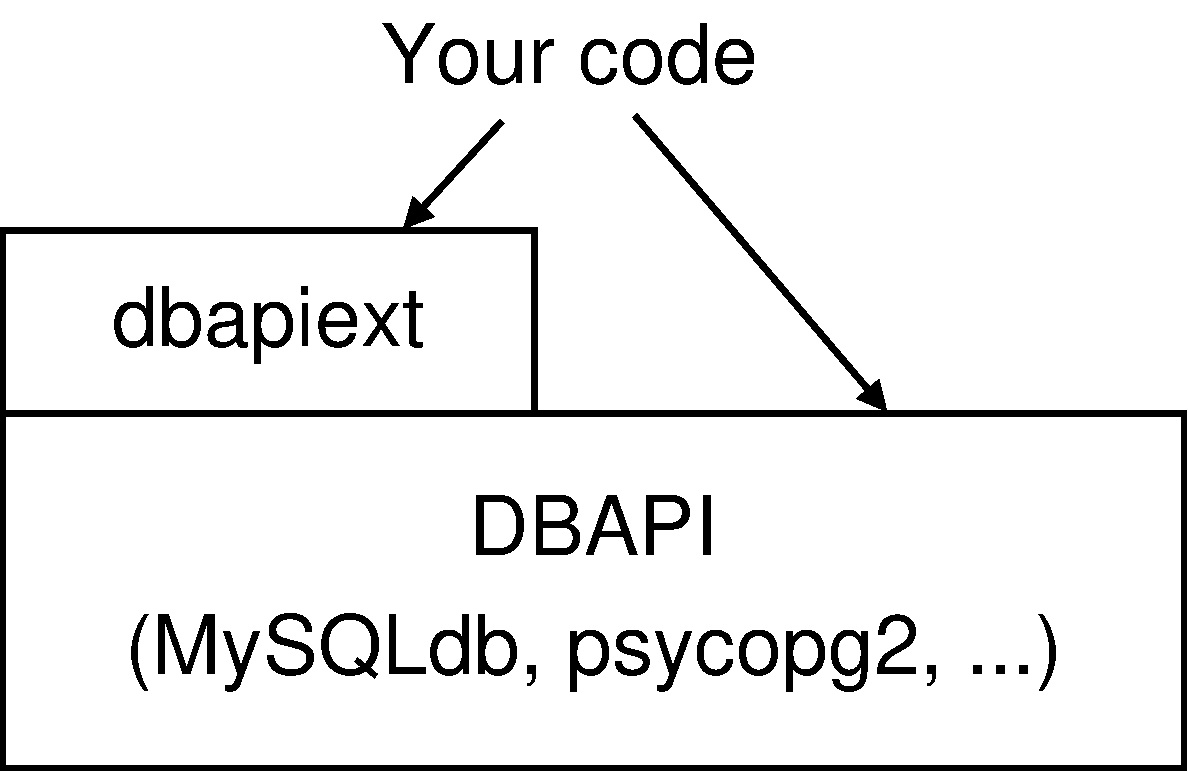
\includegraphics[width=0.4\textwidth]{layer.pdf}
  \end{center}

\end{frame}



%-------------------------------------------------------------------------------
\begin{frame}[fragile]
  \frametitle{New format specifier (\%X)}

  We provide a replacement for \texttt{execute()}, and we introduce a new format
  specifier for escaped arguments: \texttt{\%X} (capital X)

\begin{verbatim}
 cursor.execute_f(
   "INSERT INTO Users (username) VALUES (%X)",
   name)
\end{verbatim}

  You can now mix vanilla and escaped values in the arguments, and you are not
  forced to use a tuple anymore:
\begin{verbatim}
 cursor.execute_f(
   "INSERT INTO Users (%s) VALUES (%X)",
   "username", name)
\end{verbatim}

\end{frame}


%-------------------------------------------------------------------------------
\begin{frame}[fragile]
  \frametitle{Lists are Recognized and Understood}

  Lists are automatically joined with commas:
\begin{verbatim}
 columns = ["username", "email", "age"]
 cursor.execute_f("""

   INSERT INTO Users (%s) 
              VALUES (...)

  """, columns, ...)
\end{verbatim}

\begin{verbatim}

   INSERT INTO Users (username, email, age)
              VALUES (...)

\end{verbatim}

\end{frame}



%-------------------------------------------------------------------------------
\begin{frame}[fragile]
  \frametitle{Lists are Recognized and Understood}

  This also works for escaped arguments:
\begin{verbatim}
 values = ["Warren", "w@b.com", 76]
 cursor.execute_f("""

   INSERT INTO Users (%s) 
              VALUES (%X)

  """, columns, values)
\end{verbatim}

\begin{verbatim}

   INSERT INTO Users (username, email, age)
              VALUES ('Warren', 'w@b.com', 76)

\end{verbatim}

\begin{itemize}
\item Values are escaped individually and then comma-joined
\end{itemize}

\end{frame}



%-------------------------------------------------------------------------------
\begin{frame}[fragile]
  \frametitle{Dictionaries are Recognized and Understood}

  Dictionaries are rendered as required for \texttt{UPDATE} statements:
  \begin{itemize}
  \item Comma-separated \texttt{<name> = <value>} pairs
  \item Values are escaped automatically
  \end{itemize}

\begin{verbatim}
  UPDATE Lang
    SET country = 'brazil', language = 'portuguese'
    WHERE id = 3
\end{verbatim}
\vfill

\begin{verbatim}
  userid = 3
  values = {"country": "brazil",
            "language": "portuguese"}
  cursor.execute_f("""

    UPDATE Lang SET %X WHERE id = %X

  """, values, userid)
\end{verbatim}

\vfill

(Suggestion by D. Mertz)

\end{frame}


%-------------------------------------------------------------------------------
\begin{frame}[fragile]
  \frametitle{Keywords Arguments are Supported}

\begin{verbatim}
  cursor.execute_f("""

     SELECT %(table)s FROM %s
       WHERE id = %(id)X

  """, column_names, table=tablename, id=42)
\end{verbatim}

\begin{itemize}
\item Provide a useful way to recycle arguments \\
(i.e. a table or column name that occurs multiple times)

\item Positional and keyword arguments can be used simultaneously
\end{itemize}

\end{frame}



%-------------------------------------------------------------------------------
\begin{frame}[fragile]
  \frametitle{Performance and Remarks}

  \begin{itemize}
  \item The extension massages your query in a form that can be digested by
    DBAPI's \texttt{Cursor.execute()}

  \item We cache as much of the preprocessing as possible \\
(similar to \texttt{re}, \texttt{struct})
    \begin{itemize}
    \item You can cache your queries at load time with \texttt{qcompile()}.
    \end{itemize}

\pause
  \item I \emph{lied} in my examples, you have to use it like this (if
    monkey-patching \texttt{Cursor} fails):
\begin{verbatim}
   execute_f(cursor, """
      ...
\end{verbatim}

  \end{itemize}

\end{frame}



%-------------------------------------------------------------------------------
\begin{frame}[fragile]
  \frametitle{Final Thoughts}

Ideally, we would want to automatically parse the SQL queries and
determine which arguments should be quoted

  \begin{itemize}
  \item A lot more work
  \item Would have to be done at load time for performance reasons
  \end{itemize}


\end{frame}



%-------------------------------------------------------------------------------
\begin{frame}[fragile]
  \frametitle{Questions}

  \begin{center}


{\Large
\texttt{dbapiext} is part of a \\
package named \texttt{antiorm}
}

\vfill

{\LARGE
antiorm homepage: \\
\verb=http://furius.ca/antiorm/=
}

\vfill

{\LARGE Questions?}

  \end{center}

\end{frame}


%===============================================================================
\end{document}




%% %-------------------------------------------------------------------------------
%% \begin{frame}[fragile]
%%   \frametitle{Motivation (Anti-ORM Activism)}
%%
%%   \begin{center}
%%     
\includegraphics[width=0.8\textwidth]{noorms.png}
%%   \end{center}
%% \end{frame}
%%

%% %-------------------------------------------------------------------------------
%% \begin{frame}[fragile]
%%   \frametitle{Motivation}
%%
%%   \begin{quote}
%%     While some like to use ORMs to interface with databases, we prefer to
%%     maintain the full power of the SQL language, and instead focus on making the
%%     building of SQL queries much more convenient.
%%   \end{quote}
%%
%%   \begin{itemize}
%%   \item The domain-specific mini-language of SQL can never be fully replaced
%%     with an API
%%   \item ORMs hide the important facts: when does data transfer occur?  Does data
%%     get queried multiple times?
%%   \end{itemize}
%%
%% \end{frame}
%%
